\chapter{Desarrollo e implementación}
\label{chap:desarrollo}

En este capítulo se describe el desarrollo e implementación del simulador a partir del diseño presentado anteriormente. Se explica cómo se configuró el proyecto en Unity, cómo se construyó el escenario tridimensional y cómo se implementaron los elementos principales de la simulación: la reconstrucción del patrón de radiación, la generación de la rejilla de vóxeles, el cálculo de métricas mediante Python, la representación de los mapas de calor, el seguimiento de receptores móviles, la exportación de resultados y las optimizaciones de rendimiento.

\section{Configuración inicial del proyecto Unity}

La primera parte del desarrollo consiste en preparar la base sobre la que se desarrolla el simulador. Antes de implementar los cálculos de cobertura o la visualización de resultados, se debe organizar el proyecto, crear las escenas principales y preparar todos los elementos involucrados en la simulación.

El proyecto se divide en dos escenas principales: una para el menú de configuración y otra para la simulación, siguiendo la estructura definida en el capítulo anterior. Esta separación permite organizar, por un lado, los elementos de la interfaz inicial y, por otro, los componentes propios de la escena de simulación.

También se organiza la estructura de carpetas del proyecto. Los scripts se agrupan según su función en tres grupos principales: scripts del menú, scripts de configuración de la simulación y scripts de simulación. A su vez, los scripts de simulación se dividen en varios subgrupos: patrón de radiación, receptores móviles, rendimiento, rejilla de propagación, comunicación con Python y visualización.

Además, se crean carpetas específicas para otros recursos utilizados por la aplicación. Los modelos 3D se organizan en una carpeta específica, junto con carpetas separadas para prefabs, materiales, shaders, sprites y render textures. Esta separación facilita la localización de cada tipo de recurso y evita mezclar todos los recursos en una misma carpeta.

Por otro lado, se utiliza la carpeta \texttt{StreamingAssets} para guardar los recursos que deben estar disponibles durante la ejecución, como el simulador externo, el entorno Python portable, sus librerías y los archivos de entrada. Esta carpeta se mantiene tanto durante el desarrollo como después de compilar la aplicación, por lo que Unity puede acceder a estos recursos en tiempo de ejecución sin depender de rutas externas al proyecto.

También se utiliza una clase de configuración común para conservar los valores introducidos por el usuario en el menú. Cuando la configuración es válida y se carga la escena de simulación, estos valores se leen y se aplican a los componentes correspondientes. Esto permite compartir parámetros entre ambas escenas del simulador.

Con esta base preparada, el siguiente paso es la preparación del escenario donde se lleva a cabo la simulación.

\section{Desarrollo del escenario tridimensional}

A la hora de crear el escenario 3D sobre el que se lleva a cabo la simulación, en lugar de realizarse sobre un entorno urbano genérico, se decide llevar a cabo una recreación tridimensional del Centro Universitario de Mérida. Esta elección permite trabajar sobre un escenario realista aprovechando que el desarrollo del TFG se realiza en este mismo centro.

Dentro de esta recreación, la antena transmisora se sitúa en la misma zona en la que se encuentra una antena real del centro universitario. De esta forma, el escenario no solo sirve como un entorno visual, sino que también permite analizar la cobertura tomando como referencia una ubicación realista dentro del centro.

Para recrear las proporciones del Centro Universitario de Mérida, se utiliza Google Earth como referencia principal \cite{googleearth}. A partir de la vista aérea se obtienen las proporciones en planta de los edificios, carreteras, zonas verdes y el resto de elementos principales. Para estimar las alturas, se toman como referencia los valores de elevación respecto al nivel del mar proporcionados por Google Earth, calculando la diferencia entre la altura del suelo y la altura aproximada de los techos.

Esta forma de trabajar tiene algunas limitaciones. Las alturas obtenidas desde Google Earth se muestran en metros enteros, por lo que las medidas no pueden ser consideradas exactas. Además, el terreno del campus no es completamente plano, lo que introduce pequeñas diferencias de altura entre distintas zonas del mismo. Por este motivo, la topología del escenario no pretende ser una reproducción exacta, sino una aproximación lo suficientemente fiel como para utilizarse a modo de base para la simulación.

El escenario se modela íntegramente en Blender. En primer lugar, se crea un plano base para representar el terreno del campus. Este plano se divide en distintos cuadrados, ajustando la altura de cada zona según los valores de elevación obtenidos a partir de Google Earth. De esta forma, el terreno no queda completamente plano, sino que reproduce de forma aproximada los cambios de altura del entorno real.

Una vez definido el terreno base, se construyen los edificios principales del centro. Para ello, se modelan sus volúmenes partiendo de la vista en planta y de las alturas obtenidas mediante Google Earth. Posteriormente, se añaden el resto de elementos como ventanas, puertas, salientes y otros detalles visibles desde el exterior. Una vez terminados los edificios, se añaden el resto de elementos del campus, como aparcamientos, bancos, vallas o caminos.

Además de la información obtenida de Google Earth, se realizan fotografías del campus desde distintos puntos de vista. Estas imágenes no sirven como base para realizar el modelo, pero sí como apoyo para cuadrar detalles que no se aprecian correctamente desde la vista aérea, como la altura de las ventanas o puertas, las zonas entre edificios o los detalles de algunos elementos del escenario. 

En el caso de las alturas de ventanas o puertas, se realizó una aproximación realizando una regla de tres sobre las fotografías y aplicando las proporciones obtenidas sobre el modelo 3D. Este método no es del todo exacto, pues introduce un error debido a la perspectiva de las imágenes, pero es una solución razonable al no disponer de planos exteriores detallados del centro.

Tras finalizar la creación del modelo, se crearon versiones simplificadas de cada edificio usando un estilo low poly. Esto consiste en crear una réplica del edificio con una geometría más simple. En este proyecto, estas versiones se utilizan para las colisiones y la detección de obstáculos, ya que no es necesario que tengan todos los detalles visuales del modelo original. Esto es importante porque reduce la complejidad de las comprobaciones de colisión y ayuda a optimizar el simulador.

Para mejorar el aspecto visual del modelo, se utilizan texturas externas procedentes de webs como ambientCG \cite{ambientcg} y Poly Haven \cite{polyhaven}. Además, los edificios y la vegetación que rodean el campus se añaden mediante assets descargados de BlenderKit \cite{blendkit}. Estos elementos se utilizan únicamente para completar el fondo visual de la escena, por lo que no intervienen en los cálculos de propagación ni en la detección de obstáculos.

En las Figuras \ref{fig:comparacion1} y \ref{fig:comparacion2} se muestran los resultados del modelado, comparando imágenes reales del Centro Universitario de Mérida con su versión recreada en Blender.

\begin{figure}[H]
    \centering
    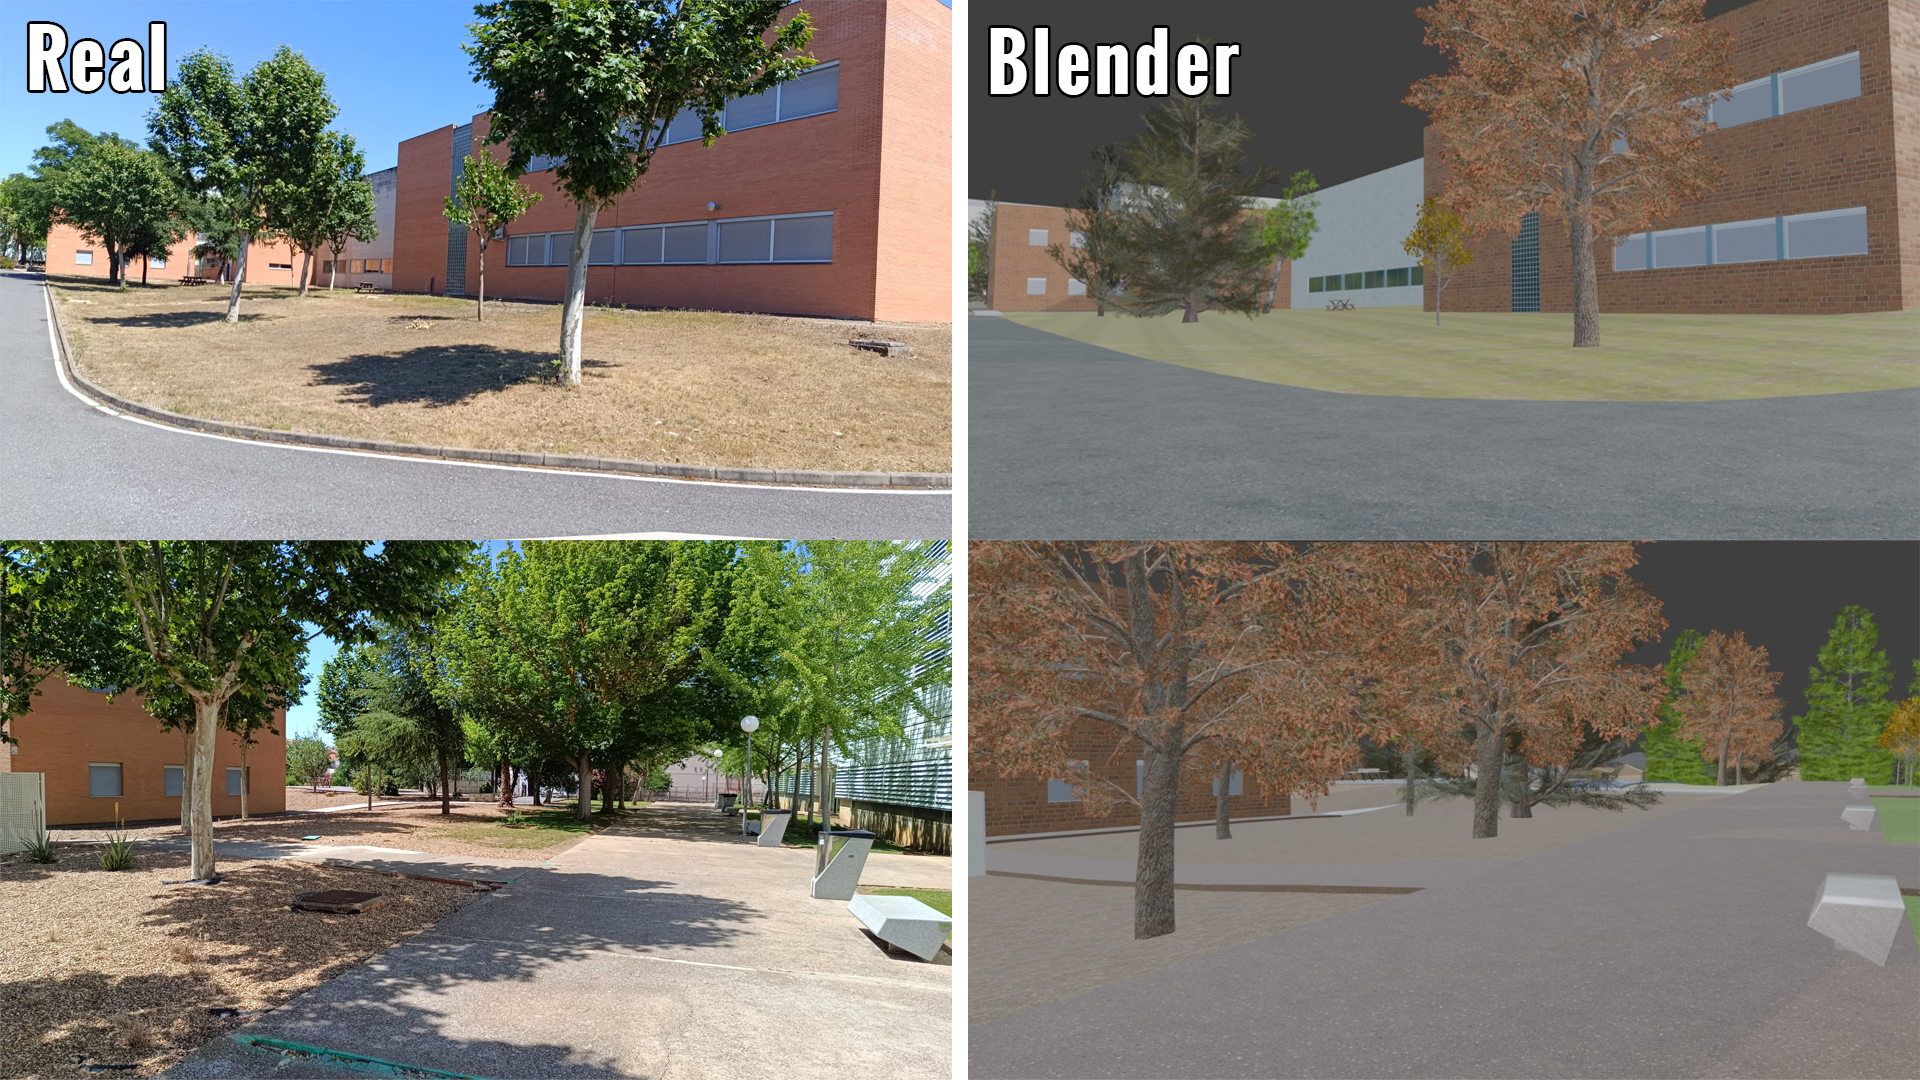
\includegraphics[width=1\textwidth, keepaspectratio]{imagenes/modelo/Comparacion1.png}
    \caption{Primera comparación entre el campus real y el modelo 3D recreado}
    \label{fig:comparacion1}
\end{figure}

\begin{figure}[H]
    \centering
    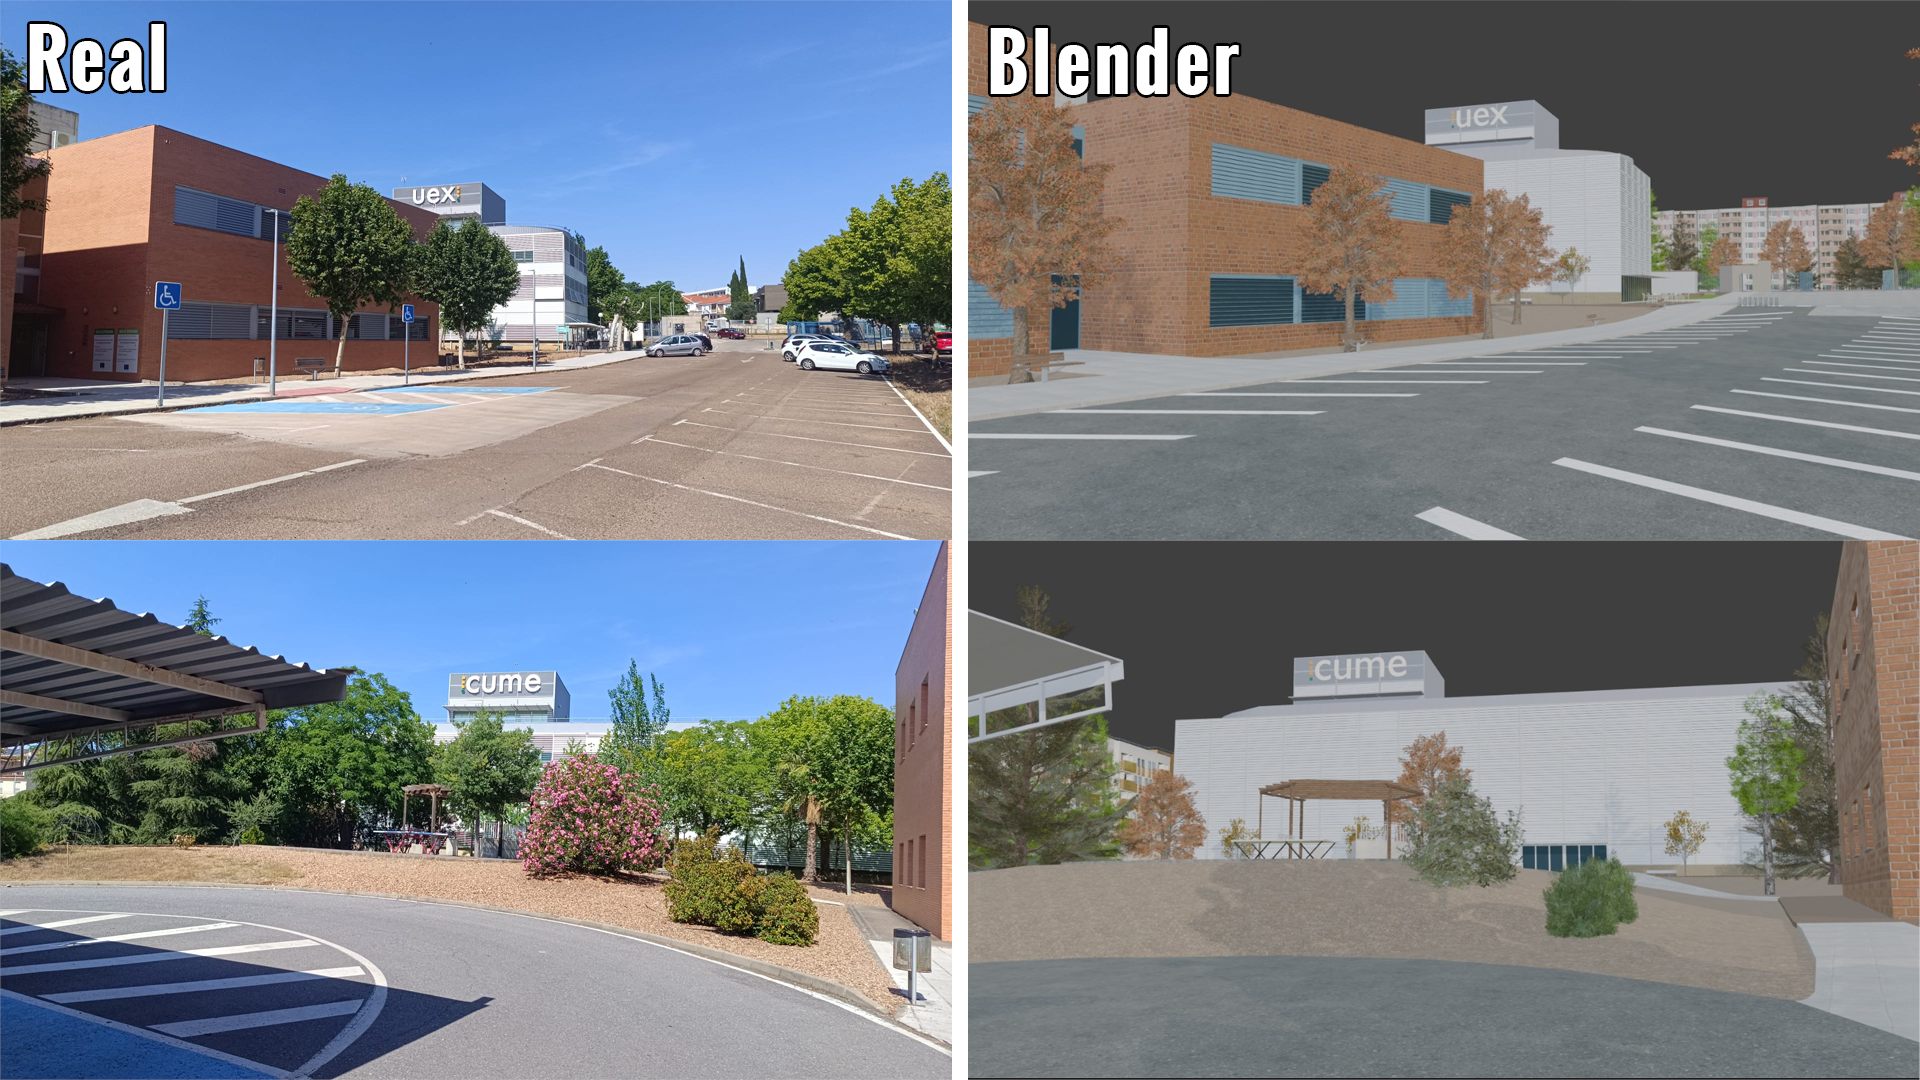
\includegraphics[width=1\textwidth, keepaspectratio]{imagenes/modelo/Comparacion2.png}
    \caption{Segunda comparación entre el campus real y el modelo 3D recreado}
    \label{fig:comparacion2}
\end{figure}

Una vez finalizado el modelo, se importa en Unity, donde se añaden la iluminación, las sombras y el cielo de la escena. El resultado final del escenario integrado en Unity se muestra en la Figura \ref{fig:escenario_unity}.

\begin{figure}[H]
    \centering
    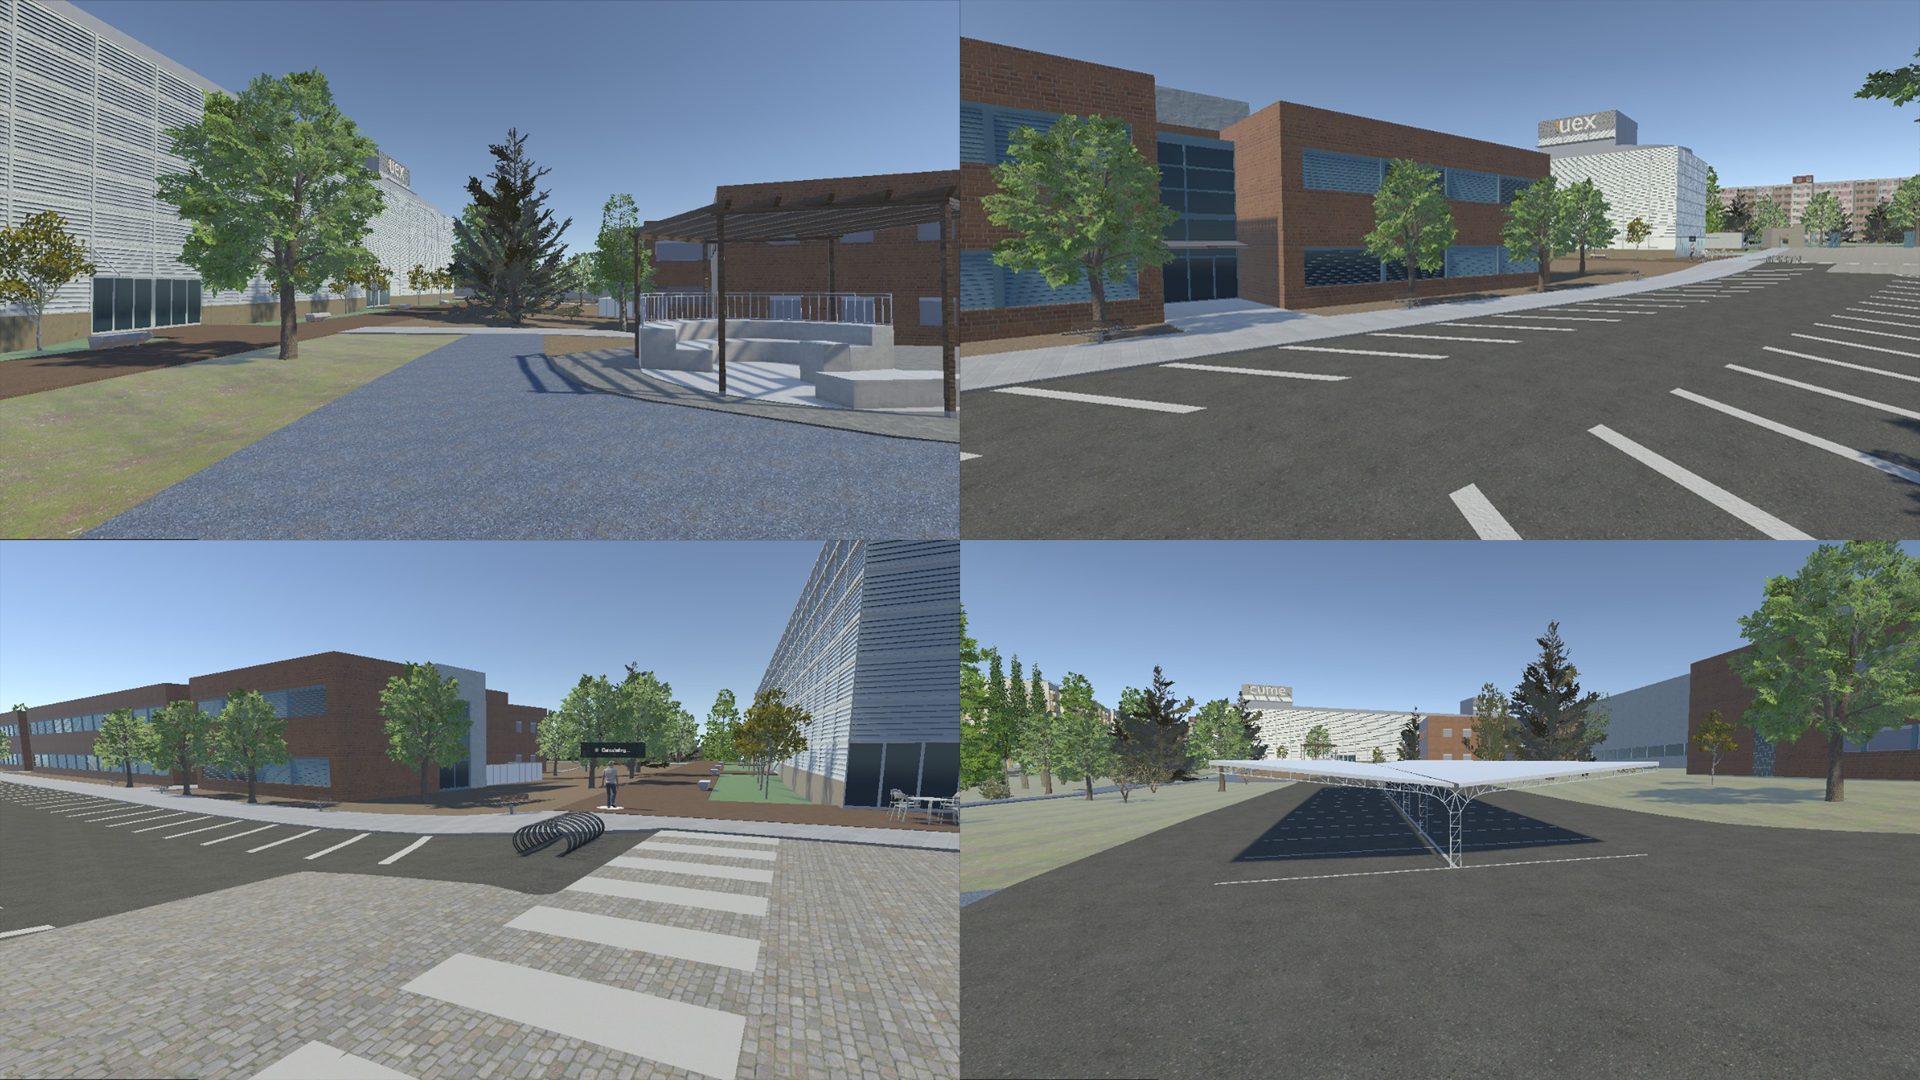
\includegraphics[width=1\textwidth, keepaspectratio]{imagenes/modelo/collage.png}
    \caption{Resultado final del escenario integrado en Unity}
    \label{fig:escenario_unity}
\end{figure}


\section{Reconstrucción del patrón de radiación de la antena}

Una vez preparado el escenario en Unity, el siguiente paso consiste en definir el comportamiento de la antena transmisora dentro de la simulación. Para ello, se implementa la reconstrucción del patrón de radiación.

En este proyecto se implementan tres modos: un patrón omnidireccional, el método de Gil y el método de Vasiliadis. El método utilizado se selecciona desde el menú de configuración, lo que permite estudiar y comparar distintos patrones de radiación.

En el caso de los métodos de Gil y Vasiliadis, la reconstrucción parte de un fichero CSV que contiene los cortes horizontal y vertical del patrón, junto con datos básicos de la antena. A partir de estos cortes, el simulador genera una matriz de ganancia tridimensional según dos ángulos: el ángulo vertical, entre 0 y 180 grados, y el ángulo horizontal o azimut, entre 0 y 359 grados.

Antes de aplicar los métodos de reconstrucción, se deben adaptar los datos del CSV de entrada. El fichero original contiene el corte vertical en función de la elevación, donde la dirección principal del patrón se encuentra a una elevación de $0^\circ$. Sin embargo, la matriz utilizada internamente en Unity representa el ángulo vertical de otra forma: $0^\circ$ corresponde a la dirección superior, $90^\circ$ al plano horizontal de la antena y $180^\circ$ a la dirección inferior.

Por esta diferencia entre referencias, el corte vertical se desplaza $90^\circ$ antes de reconstruir el patrón tridimensional. De esta forma, el máximo del corte vertical queda alineado con el plano del corte horizontal. Además, ese máximo queda centrado dentro del rango vertical utilizado por la matriz, entre $0^\circ$ y $180^\circ$, dejando una parte del patrón por encima y otra por debajo de la dirección principal.

Esta adaptación es importante para aplicar correctamente los métodos de reconstrucción. En el método de Vasiliadis, el corte vertical se utiliza dentro del rango de $0^\circ$ a $180^\circ$, mientras que en el método de Gil el patrón se separa en dos hemisferios respecto al plano horizontal. Si no se realizara este desplazamiento, el lóbulo principal quedaría en la parte superior de la matriz y los cortes horizontal y vertical no estarían alineados correctamente. Esta forma de ajustar los cortes coincide también con el criterio utilizado en las funciones de reconstrucción de patrones en MATLAB.

\par\medskip
\textbf{Nota: No puedo justificar esto último de ninguna forma, en la documentación de matlab no aparece pero, cuando usas la función en matlab, te obliga a tener el máximo en 90º. No sé si está bien dejarlo así o mejor quitar la última frase ya que no tengo referencia en la que apoyarme.}
\par\medskip

Después de alinear los cortes, se preparan los valores que se utilizarán en la reconstrucción. El CSV proporciona el patrón de radiación como atenuaciones en dB, donde la dirección principal del patrón corresponde a la menor atenuación, es decir, 0 dB. A partir de estos valores se obtiene la atenuación relativa de cada dirección.

A continuación, las atenuaciones relativas en dB se convierten a escala lineal. Con esta conversión, la dirección principal del patrón tiene valor 1 y el resto de direcciones quedan normalizadas entre 0 y 1 según su atenuación. Esta representación lineal normalizada es la que utilizan los métodos de reconstrucción para combinar los cortes. Una vez reconstruida la matriz tridimensional, los valores obtenidos se convierten de nuevo a dB relativos y se suma la ganancia máxima indicada en el CSV para obtener la ganancia absoluta en dBi de cada dirección.

El método de Gil utiliza los cortes horizontal y vertical para estimar la ganancia en cada dirección del espacio. Para ello, se separa el comportamiento del plano vertical en una parte frontal y una parte trasera, y se combinan los valores disponibles según la dirección que se quiere reconstruir. De esta forma, se obtiene una aproximación de la ganancia para cada combinación de ángulo vertical y ángulo horizontal.

El método de Vasiliadis también parte de los cortes horizontal y vertical, pero combina ambos valores mediante una ponderación controlada por un factor $k$ configurable. En la aplicación, este factor se puede modificar desde el menú de configuración cuando se selecciona este método. Esto permite ajustar cómo influyen los cortes horizontal y vertical en la reconstrucción del patrón.

Además de estos dos métodos, se implementa un patrón omnidireccional. En este caso, el patrón no se obtiene desde el CSV, sino que se genera mediante una función basada en el seno del ángulo vertical. De esta forma, la ganancia es constante en el plano horizontal y varía únicamente según el ángulo vertical. La ganancia máxima del patrón omnidireccional puede configurarse desde el menú inicial.

En el caso del patrón omnidireccional, la función senoidal utilizada hace que la ganancia sea 0 en los polos. Para evitar problemas al convertir este valor a escala logarítmica, se utiliza un límite mínimo de $10^{-12}$, equivalente a -120 dB. Este valor se mantiene en los cálculos internos, pero no se utiliza directamente para colorear el patrón de radiación. En la visualización, se limita el rango a 50 dB por debajo de la ganancia máxima, facilitando que las diferencias de ganancia sean más visibles en la representación tridimensional del patrón.

Al finalizar la reconstrucción, se generan varias matrices de ganancia. La matriz principal es la de ganancia absoluta en dBi, ya que se utiliza para calcular la ganancia transmisor-receptor, representar el color del patrón y exportar el patrón reconstruido. Además, se conserva una matriz en escala lineal normalizada, utilizada para la construcción del patrón omnidireccional tridimensional, y una matriz de ganancia relativa en dB, utilizada para pruebas internas de la aplicación.

Una vez generada la matriz de ganancia, el patrón se representa en Unity mediante un objeto tridimensional. Esta visualización permite comprobar la forma obtenida con cada método y comparar las diferencias entre el patrón omnidireccional, el método de Gil y el método de Vasiliadis. En la Figura \ref{fig:comparacion_patrones_radiacion} se muestran los tres patrones disponibles en la aplicación.

\begin{figure}[H]
    \centering
    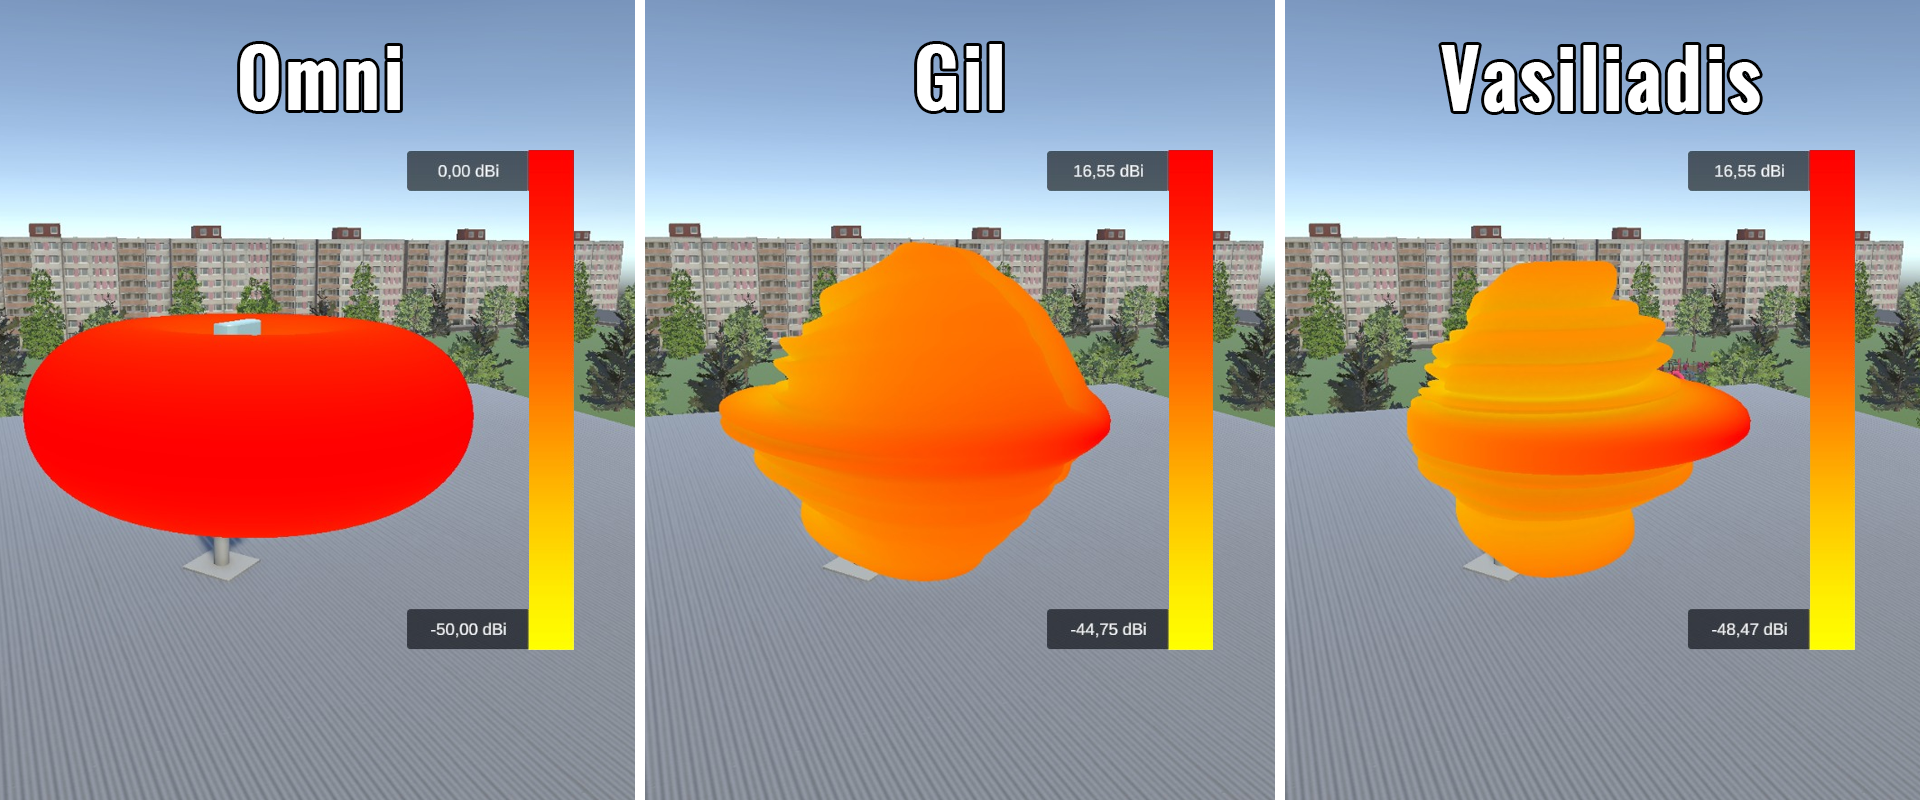
\includegraphics[width=1\textwidth, keepaspectratio]{imagenes/patron de radiacion.png}
    \caption{Comparación de los patrones de radiación implementados}
    \label{fig:comparacion_patrones_radiacion}
\end{figure}


\section{Generación de la rejilla de propagación}

Una vez reconstruido el patrón de radiación, se genera la rejilla de propagación sobre la que se calcula la potencia recibida. Esta rejilla se construye a partir de los parámetros definidos previamente en el menú de configuración: las dimensiones en los ejes X, Y y Z y el tamaño de cada vóxel.

A partir de estos valores, el simulador calcula el número de vóxeles necesario en cada eje. Además, al realizar dicho cálculo, se divide el tamaño de la rejilla entre el tamaño del vóxel y el resultado se redondea hacia arriba. De esta forma, se garantiza que el volumen configurado quede cubierto por completo, aunque las dimensiones elegidas no sean múltiplos exactos del tamaño del vóxel.

La generación de la rejilla se realiza usando la antena transmisora como referencia. Primero, se obtiene la esquina mínima del volumen en coordenadas locales de la antena, y desde esa posición se recorren los tres ejes de la rejilla. En cada iteración, se calcula la posición central del vóxel, que será el punto utilizado para realizar los cálculos posteriores.

Después, la posición central de cada vóxel se transforma a coordenadas globales de Unity, teniendo en cuenta la posición y la rotación de la antena. De esta forma, la rejilla queda orientada respecto al transmisor.

Durante todo este proceso, se almacena la información básica de cada vóxel: su índice, sus coordenadas dentro de la rejilla y su posición en el escenario. Además, para cada vóxel se preparan los datos que se enviarán posteriormente al simulador externo en Python.


\section{Cálculo de ganancias transmisor-receptor}

Tras generar la rejilla de vóxeles, se calcula la ganancia de transmisión correspondiente a cada punto de la rejilla. Esta ganancia depende del patrón de radiación reconstruido anteriormente y de la dirección entre la antena transmisora y el punto en cuestión. Para obtener esta dirección, el simulador calcula el vector que une la posición del transmisor con el centro de cada vóxel.

El vector obtenido se transforma al sistema de coordenadas local de la antena. Esto es necesario porque el patrón de radiación está definido respecto a la orientación de la antena, no respecto a los ejes globales de Unity. De esta forma, aunque la antena esté rotada dentro del escenario, la ganancia se calcula teniendo en cuenta esa rotación.

A partir de la dirección local entre la antena y el receptor, se obtienen los ángulos vertical y horizontal que definen la dirección de propagación entre ambos. Estos ángulos se utilizan para extraer el valor de la ganancia en esa dirección de la matriz de ganancias absolutas. El valor obtenido se guarda junto con la información del vóxel para utilizarse posteriormente en el cálculo de pérdidas y potencia recibida.

Además de la ganancia de transmisión, también se hace uso de la ganancia del receptor. En la rejilla de propagación se utiliza una ganancia de recepción de 0 dBi, ya que se busca obtener una referencia general de la cobertura sin asociarla a un receptor concreto.


\section{Cálculo de pérdidas, potencia recibida y SNR}

Una vez preparada la información de cada vóxel, Unity la envía al simulador externo en Python. Este simulador se encarga de calcular las pérdidas del enlace y la potencia recibida utilizando las funciones ya existentes del canal de propagación.

Para realizar estos cálculos, se utilizan los parámetros configurados en el menú inicial, como la potencia de transmisión, la frecuencia, el ancho de banda, el modelo de pérdidas, el escenario, el tipo de entorno y las ganancias de antena. La aplicación permite trabajar con modelos como FSPL o ABG, dependiendo de la configuración seleccionada por el usuario.

El simulador calcula la distancia entre el transmisor y el punto receptor y, a partir de esa distancia y del modelo seleccionado, obtiene las pérdidas del canal. Además, cuando Unity proporciona una pérdida adicional por edificios, esta se suma a las pérdidas base del modelo de propagación.

Con las pérdidas totales del enlace, la potencia de transmisión y las ganancias de antena, el simulador calcula la potencia recibida mediante el presupuesto de potencia implementado en Python. En la rejilla de propagación se devuelve para cada vóxel la distancia, las pérdidas y la potencia recibida, ya que estos valores son los necesarios para construir el mapa de calor.

La SNR no se calcula para la rejilla de propagación, ya que el mapa de calor busca representar una referencia general de la potencia recibida en el escenario, sin asociarla a un tipo de comunicación concreto ni a un ancho de banda específico. En cambio, en los receptores móviles sí se calcula esta métrica, ya que representan casos concretos de comunicación, como receptores celulares 5G o V2X. Para obtenerla, se utiliza la función de SINR del simulador externo, introduciendo las interferencias con valor cero, ya que en este proyecto solo se utiliza un transmisor.


\section{Detección de obstáculos y pérdidas por edificios}

Para tener en cuenta la presencia de edificios entre el transmisor y los receptores, se implementa un sistema de detección de obstáculos en Unity. Este sistema permite añadir una pérdida adicional cuando la señal atraviesa edificios antes de llegar al receptor en cuestión.

Para ello, además del modelo del escenario, se crean en Blender versiones simplificadas de los edificios destinadas únicamente a las colisiones. En Unity, un \textit{collider} es el volumen que se utiliza para detectar contactos o intersecciones con otros objetos, aunque no tiene por qué coincidir exactamente con la geometría del modelo. En este caso, los \textit{colliders} de los edificios se utilizan para saber si la línea entre el transmisor y el receptor atraviesa algún edificio.

Estas versiones de colisión tienen una geometría más simple que representa el volumen de cada edificio. En edificios con formas más complejas, como el aulario, el modelo se divide en varias piezas. Esto es fundamental porque, si todo el edificio se representara como un único \textit{collider}, un rayo que atravesara varias zonas del mismo edificio se contabilizaría como una única colisión. Al dividirlo en prismas rectangulares, se consigue detectar los distintos tramos atravesados por la señal.

La detección se realiza mediante \textit{raycasting}. Para cada punto receptor, se construye el segmento que une la antena transmisora con dicho punto. A continuación, Unity lanza un rayo sobre ese segmento y obtiene los \textit{colliders} de edificios que son atravesados. Todos estos \textit{colliders} están etiquetados como edificios, de forma que no se tienen en cuenta otros elementos visuales del escenario.

Sin embargo, al dividir un edificio en varios prismas puede aparecer un problema adicional. Un mismo tramo atravesado por la señal puede pasar por varios \textit{colliders} consecutivos que forman parte del mismo edificio o de una misma zona continua. Si se contara cada impacto del rayo por separado, se podrían añadir más pérdidas de las que corresponden. Por este motivo, se implementa un algoritmo que no se basa únicamente en el número de impactos detectados, sino en los tramos reales atravesados por la señal. El algoritmo implementado se muestra a continuación:

\begin{algorithm}[H]
\caption{Cálculo de colisiones con edificios}

\KwIn{Posición del transmisor y posición del receptor}
\KwOut{Número de colisiones con edificios}
Crear el segmento transmisor-receptor\;
Obtener mediante raycasting los colliders de edificios atravesados\;
Inicializar la lista de tramos ocupados por edificios\;

\For{cada collider atravesado}{
    Calcular el punto de entrada del rayo en el collider\;
    Calcular el punto de salida del rayo en el collider\;
    Guardar el tramo ocupado por ese collider dentro del segmento\;
}
Ordenar los tramos ocupados según su distancia al transmisor\;
Fusionar los tramos solapados o consecutivos\;
Calcular el número de colisiones con edificios a partir de los tramos resultantes\;

\Return{colisiones}

\end{algorithm}

El algoritmo calcula, para cada \textit{collider} atravesado, el tramo del segmento transmisor-receptor que queda dentro del edificio. Para ello, se lanza un rayo desde el transmisor hacia el receptor para obtener el punto de entrada y otro desde el receptor hacia el transmisor para obtener el punto de salida. Con ambos puntos se define el tramo ocupado por ese \textit{collider}.

Una vez obtenidos todos los tramos ocupados, estos se ordenan y se fusionan cuando se solapan o están conectados. De esta forma, varios \textit{colliders} consecutivos que representan una misma zona atravesada se interpretan como un único tramo real. Cada tramo continuo se cuenta como una entrada y una salida del edificio, por lo que normalmente equivale a dos colisiones con edificios. Si el punto receptor queda dentro del edificio, se elimina la colisión de salida, ya que la señal entra en el edificio pero no llega a salir antes de alcanzar el receptor.

La pérdida adicional por edificios se calcula multiplicando el número de colisiones por una pérdida fija por pared. Para esta pérdida se utiliza como referencia la especificación ETSI TR 138 901, que contiene las pérdidas por penetración de distintos materiales. En el caso del hormigón, la pérdida se calcula como $L_\mathrm{concrete} = 5 + 4f$ dB, asumiendo un grosor de 23 cm y siendo $f$ la frecuencia en GHz \cite{etsi138901}.

En este proyecto se considera que los edificios del escenario son construcciones de hormigón, por lo que se aplica la expresión anterior para estimar la pérdida añadida por cada colisión.

Finalmente, esta pérdida se suma a las pérdidas obtenidas mediante el modelo de propagación seleccionado. De esta forma, el cálculo de potencia recibida no depende únicamente de la distancia y del modelo de canal, sino también de si la señal atraviesa edificios dentro del escenario tridimensional.


\section{Mapa de calor 3D y 2D}

Una vez recibidos los resultados calculados por Python, Unity construye la representación gráfica correspondiente a la rejilla de potencia recibida. Para ello, se utiliza el valor de potencia recibida de cada vóxel y se normaliza utilizando los valores mínimo y máximo obtenidos.

Aunque cada vóxel se visualiza como un pequeño cubo dentro del mapa de calor 3D, no se crea un objeto independiente para cada uno de ellos. Tener un objeto por cada vóxel significaría generar una gran cantidad de objetos en la escena, lo que afectaría notablemente al rendimiento.

Para mejorar el rendimiento ante un gran número de vóxeles, se agrupan en bloques o \textit{chunks}. Cada \textit{chunk} está formado por un conjunto de vóxeles cercanos dentro de la rejilla y se representa mediante una única malla asignada a un solo objeto. En el contexto de los modelos 3D, una malla es una estructura formada por vértices, aristas y caras, que permite representar objetos tridimensionales. De esta forma, se reduce el número de objetos que Unity debe manejar y se mejora el rendimiento. La malla de cada \textit{chunk} se construye a partir de los cubos visibles que forman parte de ese bloque.

Cada vóxel visible se representa como un cubo centrado en la posición calculada durante la generación de la rejilla. El color se obtiene a partir de la potencia recibida normalizada, utilizando tonos más cercanos al rojo para valores altos y tonos más cercanos al negro para valores bajos. Además del color, se calcula una transparencia para cada vóxel a partir de los parámetros configurados por el usuario.

La transparencia final se obtiene a partir de la transparencia mínima, la transparencia máxima y el exponente de transparencia. Estos valores permiten modificar la opacidad de cada vóxel según su potencia recibida, haciendo menos visibles las zonas de baja potencia y destacando las regiones con mayor señal.

El umbral de visualización se aplica sobre la potencia recibida normalizada. Los vóxeles cuyo valor queda por debajo del umbral seleccionado no se incluyen en la malla final, por lo que dejan de mostrarse en el mapa de calor. Cuando el usuario modifica el slider de umbral, el valor se muestra también en dBm y, al soltar el control, se reconstruyen los \textit{chunks} visibles del mapa. En la Figura \ref{fig:heatmap_umbral} se muestra un ejemplo del mapa de calor 3D saturado por un exceso de vóxeles y a su lado el mismo mapa con el umbral aplicado.

\begin{figure}[H]
    \centering
    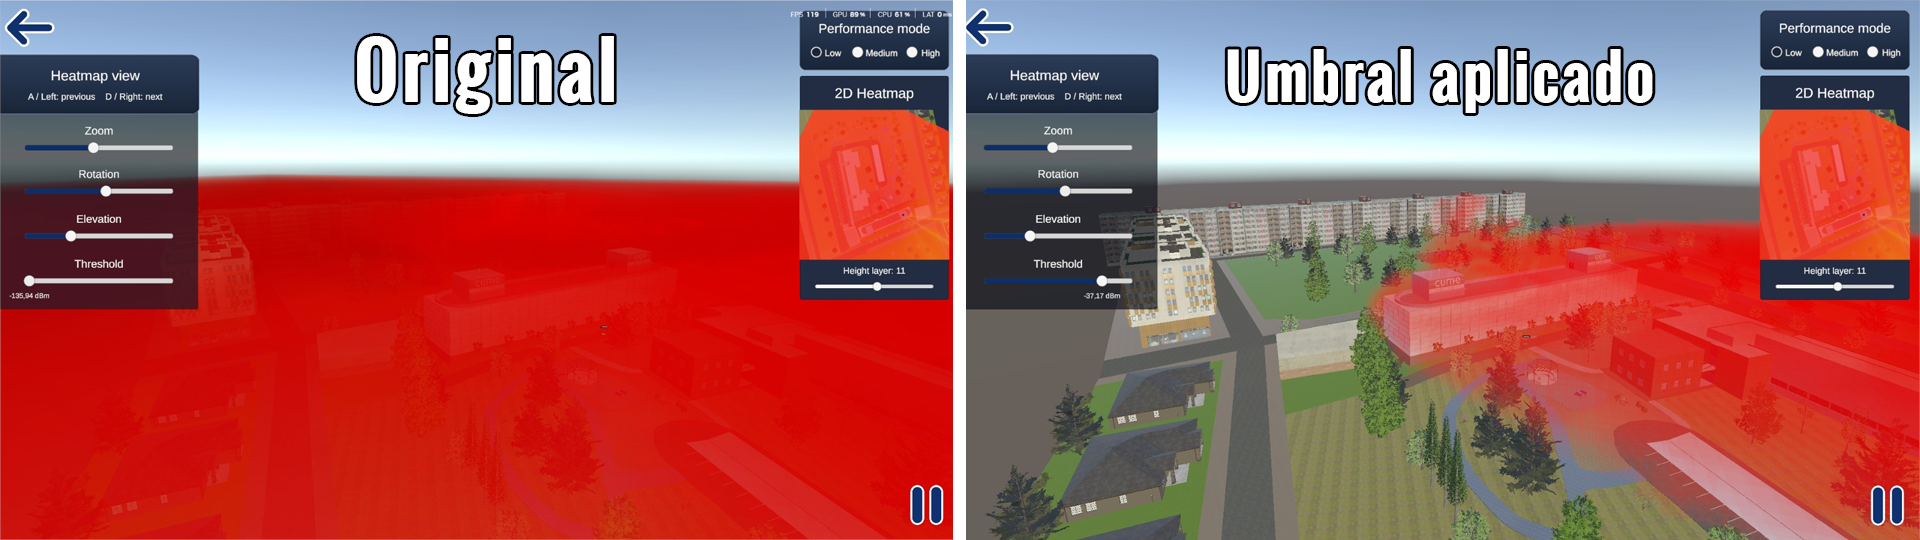
\includegraphics[width=1\textwidth, keepaspectratio]{imagenes/mapas de calor/umbral.png}
    \caption{Mapa de calor 3D con umbral de visualización aplicado}
    \label{fig:heatmap_umbral}
\end{figure}

Además del mapa 3D, se implementa una versión 2D por capas. Esta vista utiliza los mismos datos de la rejilla, pero muestra únicamente los vóxeles pertenecientes a una altura concreta. El usuario puede seleccionar la capa mediante un slider, y la textura del mapa se actualiza para mostrar la distribución de potencia recibida a esa altura.

Para generar el mapa 2D, se crea una textura sobre la que se pintan los vóxeles de la capa seleccionada. Cada vóxel se proyecta sobre el plano del mapa y se colorea según su potencia recibida normalizada. Como la rejilla puede estar rotada respecto al escenario, se calculan las esquinas del vóxel en el plano 2D y se rellena el área de píxeles correspondiente. 

Para evitar huecos visuales debidos al redondeo, se utiliza redondeo hacia abajo en los valores mínimos y redondeo hacia arriba en los valores máximos del área ocupada. Esta solución evita que queden espacios vacíos entre vóxeles debido al redondeo, aunque puede producir dientes de sierra en el minimapa 2D cuando el tamaño de vóxel utilizado es grande.

La vista 2D se genera a partir de una cámara ortográfica situada sobre el campus, que muestra una vista cenital del escenario. Para definir qué zona del escenario debe aparecer en esta imagen se utilizan dos puntos de referencia colocados en la escena, que marcan los límites del mapa. A partir de esos mismos límites, las posiciones de los vóxeles en coordenadas del mundo se convierten a coordenadas de píxel, permitiendo dibujar el mapa de calor exactamente sobre la zona correspondiente de la imagen cenital. De esta forma, el usuario puede relacionar la distribución de potencia recibida con los edificios, caminos y zonas del entorno. En la Figura \ref{fig:heatmap_2d_capas} se muestra un ejemplo del mapa de calor 2D por capas.

\begin{figure}[H]
    \centering
    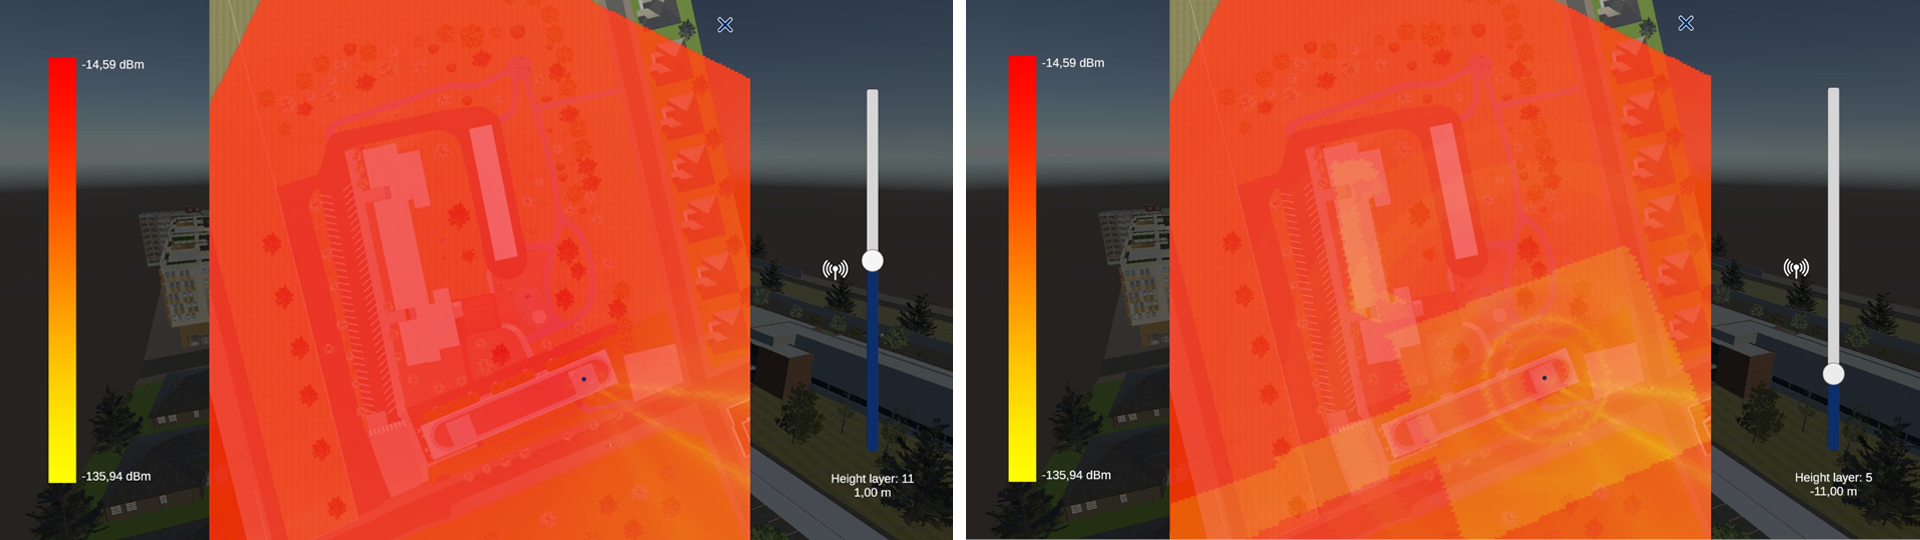
\includegraphics[width=1\textwidth, keepaspectratio]{imagenes/mapas de calor/mapa de calor 2d varias alturas.png}
    \caption{Mapa de calor 2D por capas}
    \label{fig:heatmap_2d_capas}
\end{figure}


\section{Receptores móviles, rutas y métricas}

Los receptores se desplazan por el escenario siguiendo rutas definidas previamente mediante puntos colocados en Unity. Cada ruta representa un tipo de recorrido diferente dentro del campus. De esta forma, la simulación no solo calcula la cobertura en puntos fijos, sino que también permite estudiar cómo varía la señal durante un recorrido.

En este trabajo se utilizan tres receptores móviles: un vehículo que recorre el campus, un vehículo con un recorrido lineal hacia la antena y un peatón. Al disponer de varios recorridos distintos, se pueden observar diferentes situaciones dentro del mismo escenario. El vehículo del campus representa un desplazamiento completo por todo el campus, el vehículo lineal permite analizar la evolución de la señal de forma lineal, y el peatón representa un caso de movimiento de un dispositivo 5G dentro del propio campus.

Cada receptor tiene asociada una ruta y una velocidad de movimiento en m/s. Durante la simulación, el receptor avanza de un punto de la ruta al siguiente. Al llegar a un punto, continúa hacia el siguiente hasta completar el recorrido. En el caso del vehículo del campus y el peatón, ambos realizan su ruta en bucle de forma ilimitada. No obstante, el vehículo lineal se detiene al llegar al final y se queda estacionado.

Los receptores también utilizan una ganancia de recepción configurable desde el menú inicial. Los vehículos emplean la ganancia definida para receptores vehiculares, mientras que el peatón utiliza la ganancia definida para receptores celulares. De esta forma, los valores pueden modificarse en función del caso que se quiera estudiar.

El movimiento de los receptores no comienza nada más cargar la escena. Antes de activarlos, el simulador espera a que se haya generado la rejilla de propagación y a que el servidor Python esté preparado para recibir peticiones. De esta forma, se evita que los receptores empiecen a recorrer la escena antes de que puedan calcular sus métricas.

Una vez que el sistema está preparado, se activa el movimiento de los receptores y comienza el registro de muestras. Durante el recorrido, Unity solicita periódicamente al servidor Python las métricas de cada receptor a partir de su posición actual. En la escena, esta actualización se realiza cada 0,05 segundos, por lo que se obtiene una secuencia de valores de potencia recibida, SNR, distancia al transmisor y pérdidas del enlace.

El registro de datos se detiene cuando el receptor completa su primer recorrido. Esto evita mezclar varias vueltas en una misma gráfica, ya que los datos serían equivalentes. Si la simulación se interrumpe antes de que un receptor termine su ruta, se exportan las muestras registradas hasta ese momento, evitando que se pierdan los datos obtenidos.

\section{Paneles de métricas y visualización de cobertura}

Los receptores móviles cuentan con paneles de métricas que muestran los valores calculados durante la simulación. Con cada nueva respuesta recibida desde Python se actualizan los valores mostrados en la interfaz, como la distancia al transmisor, la potencia recibida, la SNR, las pérdidas del enlace y el número de colisiones con edificios.

Junto con el panel de métricas, se implementa un visualizador de cobertura asociado a cada receptor móvil. Este visualizador muestra el estado de la cobertura a partir de la SNR obtenida en cada actualización. A primera vista, podría pensarse que el único umbral necesario es 0 dB, ya que la SNR representa la relación entre la potencia de señal y el ruido. En escala logarítmica, una SNR de 0 dB indica que la potencia de señal y la potencia de ruido son iguales, mientras que valores positivos indican que la señal está por encima del ruido.

Sin embargo, para representar la calidad de cobertura de forma más útil, no basta con distinguir únicamente entre valores positivos y negativos. Por este motivo, se buscó una referencia orientativa que permitiera separar distintos niveles de calidad de señal. La documentación de Cisco sobre resolución de problemas en interfaces celulares proporciona una tabla con rangos de calidad para RSSI, RSRP, RSRQ y SNR \cite{cisco_troubleshooting_cellular}. A partir de esa tabla se toman como referencia los límites de SNR de 20 dB, 13 dB y 0 dB.

Con estos umbrales se definen cuatro estados de cobertura: excelente para valores de SNR mayores o iguales que 20 dB, buena para valores entre 13 dB y 20 dB, aceptable para valores entre 0 dB y 13 dB, e insuficiente para valores menores que 0 dB. Estos límites no se interpretan como norma absoluta, sino que se utilizan como criterio visual para facilitar la interpretación de la cobertura durante la simulación.

El visualizador de cobertura está formado por un mensaje sobre el receptor y un indicador circular en el suelo. Cada vez que se reciben nuevas métricas, el sistema actualiza el texto y el color del indicador según el estado de cobertura calculado. De esta forma, el usuario puede identificar rápidamente la calidad del enlace sin depender únicamente del panel numérico.

\section{Generación automática de CSV y gráficas}

La generación de resultados se realiza durante la ejecución de la simulación. Cada receptor móvil tiene una lista con las muestras obtenidas durante su recorrido. De esta forma, los datos de los receptores no se mezclan entre sí y pueden exportarse de manera separada.

El registro de muestras comienza cuando la escena ya está preparada y los receptores empiezan a desplazarse. Cada vez que se reciben nuevas métricas desde el simulador Python, se guarda una muestra asociada al receptor correspondiente. 

Cuando un receptor completa su primer recorrido, se exportan las muestras almacenadas en un archivo CSV. Cada archivo contiene una cabecera con el nombre de las columnas y una fila por cada muestra registrada. Este archivo utiliza la coma como separador entre columnas y el punto como separador decimal. Además, los valores reales se guardan con tres decimales para facilitar su procesado posterior.

Una vez exportado el CSV de un receptor, se generan automáticamente las gráficas seleccionadas por el usuario en el menú de configuración. Para ello se utiliza el entorno Python integrado, que lee los datos exportados y crea las imágenes correspondientes en la misma carpeta de resultados.

Las gráficas generadas permiten analizar la potencia recibida y la SNR respecto a la distancia al transmisor, además de la evolución de la SNR respecto al tiempo. En esta última se añaden las líneas de los umbrales configurados y se calcula el porcentaje de tiempo en el que el receptor se mantiene por encima del límite de cobertura.

Además de exportar los resultados cuando un receptor completa su recorrido, la aplicación también tiene en cuenta el caso en el que la simulación se interrumpa antes de terminar. Si el usuario vuelve al menú o cierra la aplicación, se exportan igualmente las muestras disponibles hasta ese momento, evitando que se pierdan los datos ya registrados.

\section{Optimización y modos de rendimiento}

Durante el desarrollo del simulador, se añaden varias medidas para adaptar la aplicación a equipos con distintas capacidades. La escena principal está formada por un modelo tridimensional del campus, mapas de calor, receptores móviles, paneles de interfaz y comunicación periódica con el servidor Python, por lo que el rendimiento puede variar bastante según el ordenador utilizado.

Además de las optimizaciones de la representación del mapa de calor explicadas anteriormente, se añadieron modos de rendimiento configurables desde la interfaz. Estos modos permiten activar o desactivar elementos secundarios del escenario. En el modo de bajo rendimiento, se muestra el escenario completo. En el modo intermedio se oculta la vegetación, y en el modo de mayor rendimiento se ocultan la vegetación, el parque y los edificios de fondo.

Estos elementos mejoran el aspecto visual de la escena, pero no intervienen en los cálculos de propagación. Por este motivo, pueden desactivarse sin modificar los resultados de la simulación. De esta forma, el usuario puede reducir la carga gráfica cuando el dispositivo no sea capaz de ejecutar la escena con fluidez.

Otra medida aplicada es la limitación de los fotogramas por segundo (FPS). Sin esta limitación, la aplicación intenta generar el mayor número de FPS posible, aumentando innecesariamente el uso de CPU y GPU. Para evitarlo, se establece un límite en función de la frecuencia de refresco del monitor, pero sin superar los 120 FPS.

Con esta solución, en un monitor de 60 Hz, la aplicación se limita a 60 FPS, mientras que en monitores de mayor frecuencia se permite una tasa superior, hasta un máximo de 120 FPS. Esto evita fijar la aplicación a 60 FPS, lo que podría desaprovechar la fluidez de los monitores actuales, pero también impide que la simulación consuma recursos excesivos intentando alcanzar tasas de fotogramas demasiado altas.
